%\setcounter{equation}{0}
\chapter{Introdução}
usar o texto como referência.
No Brasil, a eletricidade é gerada por hidrelétricas, termoelétricas, parques eólicos e usinas nucleares. Na maioria dos casos, devido a condições geográficas e de segurança, a energia gerada nem sempre é utilizada ou consumida no local de sua geração. Portanto, há a necessidade do uso de linhas de transmissão para transportar energia gerada na fonte geradora para a carga do consumidor (Brandão, 2009). O mercado consumidor brasileiro é composto de cerca de 47 milhões de unidades. Em termos de linhas de transmissão de energia, são cerca de 77.640 km, que devem estar operando 24 horas por dia, 7 dias por semana, 365 dias por ano e em perfeito estado de manutenção, para garantir eletricidade para os consumidores (ONS, 2006).
No Brasil, há uma quantidade considerável de linhas de transmissão de alta tensão que já ultrapassaram a vida útil as quais foram destinadas. Com o envelhecimento dos cabos, a inspeção para manutenção preventiva é um fator de extrema relevância para garantir o perfeito funcionamento dos sistemas elétricos. 
De um modo geral, as inspeções nas linhas de transmissão de alta tensão são realizadas regularmente de forma visual, a fim de identificar a necessidade da realização de manutenções preventivas. 
As inspeções buscam verificar a integridade física dos componentes das linhas, em termos de fissuras, corrosão e eventuais danos que venham a prejudicar o fornecimento de energia elétrica. Essas inspeções envolvem a análise da integridade estrutural das torres, da condição dos isoladores, das conexões das linhas de transmissão, dentre outros, a fim de se verificar a existência de eventuais pontos de ruptura. 
Um dos métodos empregados para detecção de pontos quentes nos cabos é o imageamento térmico, que é capaz de identificar uma elevação de temperatura nos cabos, o que é um indício de possíveis pontos de ruptura. A inspeção através de câmera térmica é uma importante ferramenta no campo das inspeções para manutenções preventivas. 
Outros pontos a serem inspecionados envolvem as condições do local onde as torres são instaladas, pois a vegetação e eventuais construções devem ser mantidas a uma distância mínima segura, tal que não ocorra nenhum contato entre quaisquer estruturas e as torres ou cabos de transmissão, evitando assim interferências no funcionamento da linha. 
Além disso, é essencial a garantia de dispor-se de um terreno em condições de trânsito de veículos para o transporte do pessoal de manutenção, transporte de ferramentas, dentre outros fatores. 
Durante vários anos, a inspeção de linhas de transmissão de alta tensão tem sido feita regularmente através de aeronaves tripuladas. As aeronaves executam vôos em baixa altitude e muito próximos das linhas de transmissão conforme mostrado na  Figura 1 (Rangel, Kienitz, Brandão, 2009).
%%%%%%%%%%%%%%%%%%%% PICTURE %%%%%%%%%%%%%%%%%%%%%%%%%%%%%%%
\begin{figure} [h!]												% Begin of the figure
	\centering													% Centering the figure
	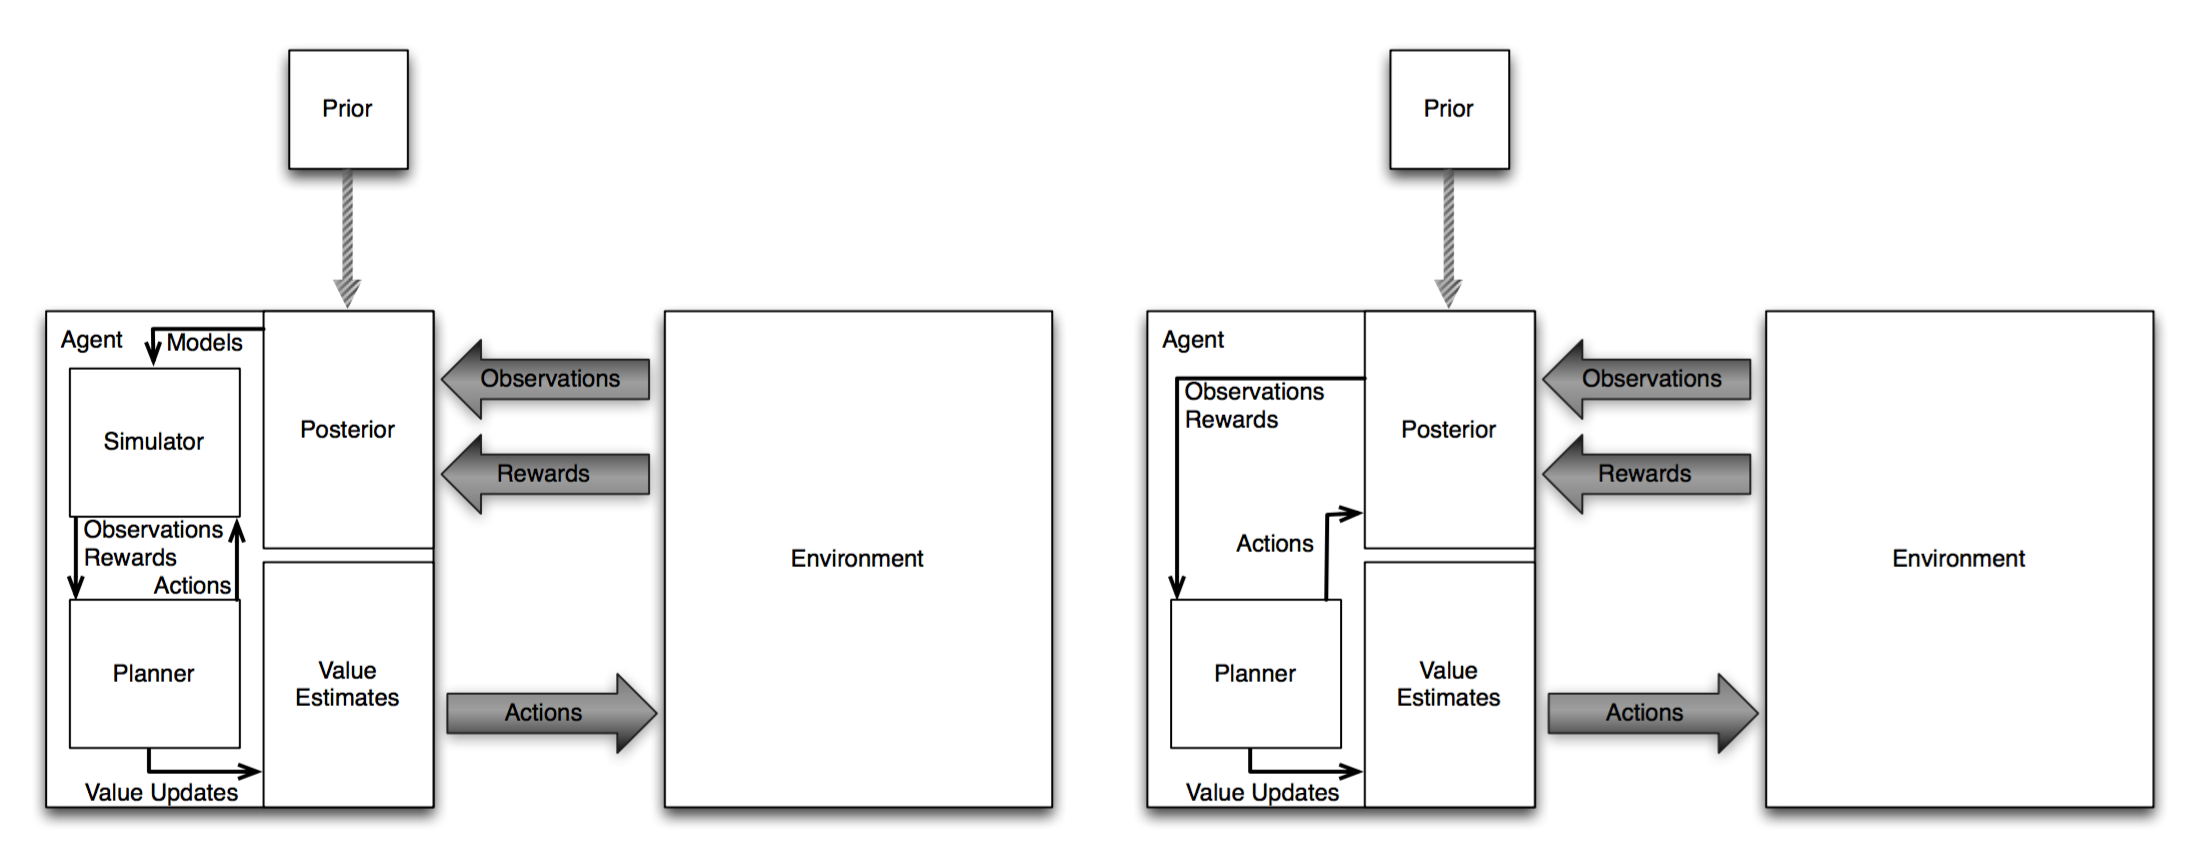
\includegraphics[width=1.0\textwidth]{./asmuth}				% Including picture
	\caption{Inspeção de linhas de transmissão feita por aeronaves tripuladas. \cite{asm:13}.}			% Including title
	\label{asmuth}												% Caption of the figure
\end{figure}													% End of the figure
%%%%

Em alguns casos, devido às características geográficas da região, condições climáticas e outros fatores que venham a dificultar o sobrevôo, há uma grande exposição dos tripulantes a riscos associados à tarefa. Além dos perigos aos quais os tripulantes são expostos, a inspeção feita com aeronaves tem um custo bastante elevado. Outra forma alternativa de inspeção é o uso de veículos terrestres, porém essa forma é muito limitada, pois boa parte das linhas de transmissão está localizada em áreas de difícil acesso terrestre, muitas vezes restritas pelas características geográficas da região. Além disso, o ângulo de visão é, muitas vezes, desfavorável para a realização da inspeção.

Outra maneira de inspecionar as linhas de transmissão é através de eletricistas que literalmente caminham sobre os cabos de linhas de transmissão de alta tensão (Figura 2), realizando inspeção visual e termográfica. Esse tipo de inspeção é lenta e não é viável, tendo em vista que o país possui milhares de quilômetros de linhas de transmissão.
%%%%%%%%%%%%%%%%%%%% PICTURE %%%%%%%%%%%%%%%%%%%%%%%%%%%%%%%
\begin{figure} [h!]												% Begin of the figure
	\centering													% Centering the figure
	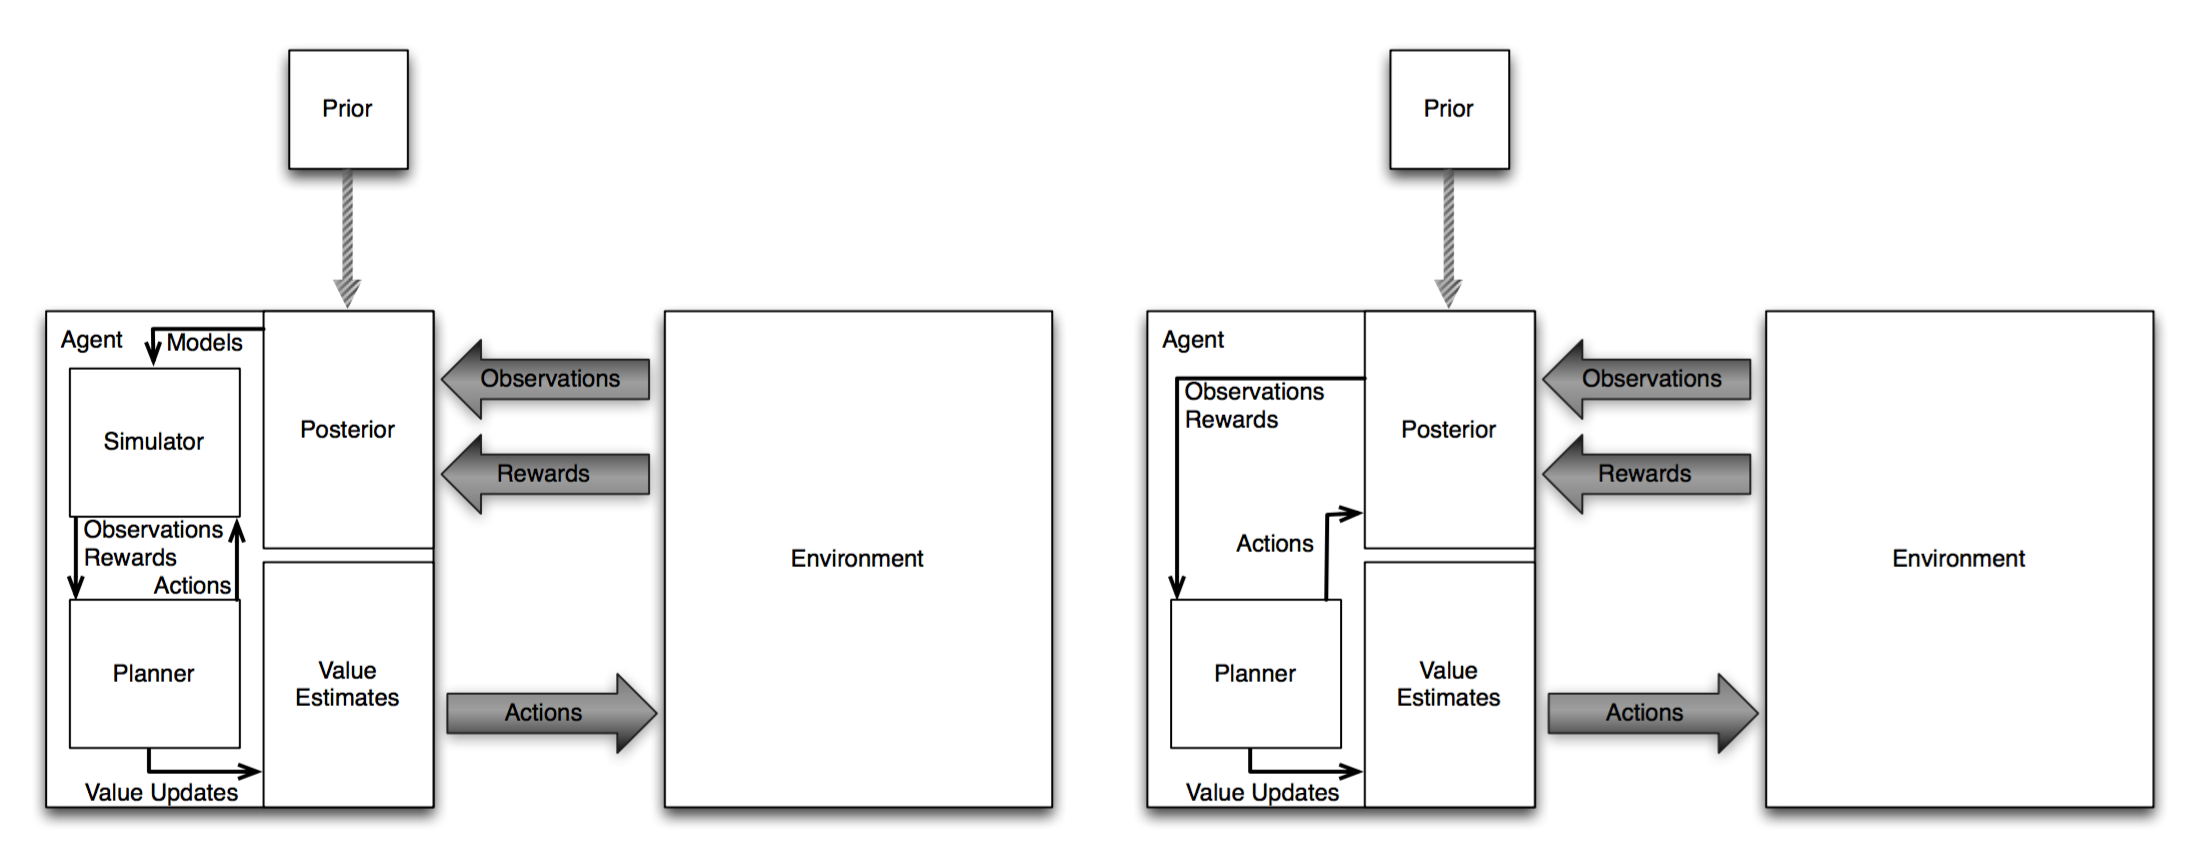
\includegraphics[width=1.0\textwidth]{./asmuth}				% Including picture
	\caption{Inspeção de linhas de transmissão feita por aeronaves tripuladas. \cite{asm:13}.}			% Including title
	\label{asmuth}												% Caption of the figure
\end{figure}													% End of the figure
%%%%

Neste contexto vários robôs de inspeção de linhas de transmissão foram desenvolvidos, porém poucos deles consistiram em projetos de engenharia que sejam aplicáveis no mundo real, além disso a maioria eram robôs teleoperados, ou seja robôs controlados por seres humanos. Um dos pontos diferenciais deste projeto de tese é a proposição de um desenvolvimento de uma navegação autônoma utilizando técnicas de aprendizagem de máquinas até então não utilizadas em robôs de inspeção de linhas de transmissão de alta tensão.

\section{Objetivos}
Neste contexto o objetivo principal deste projeto de tese será o de simular um ambiente de inspeção a ser realizado por um robô, onde o mesmo seja capaz de navegar de forma autônoma detectando e transpondo os objetos e tentos partidos encontrados na linha de transmissão de alta tensão. Durante a etapa de detecção o robô deverá ser capaz de reconhecer um ponto quente nos cabos ou nos objetos e fotografá-los, além disso durante o processo de inspeção e navegação o robô deverá realizar uma filmagem da faixa de servidão referenciando geometricamente a posição e coletando informações da distância entre a linha de transmissão e o obstáculo mais próximo em relação ao solo.


\section{Objetivos específicos}
O objetivo do projeto de tese será o desenvolvimento, em três anos, de uma simulação de um robô com navegação autônoma, com as seguintes características:
\begin{itemize}
\item capacidade de deslocar-se em linha de transmissão de alta tensão e transpor objetos, tais como cadeia de isoladores, esferas de sinalização, estabilizadores, jumpers e outros componentes;
\item funcionamento independente de operadores;
\item propulsão realizada com motores elétricos, movidos por bateria	;
\item sensores de temperatura e termógrafos para levantamento dos pontos quentes e da temperatura do cabo;
\item câmeras de espectro visível para inspeção visual da linha, cadeia de isoladores e faixa de servidão;
\item características mecânicas compatíveis com os movimentos necessários para o deslocamento na linha de transmissão;
\item sistema mecânica de baixo peso e design que permita um procedimentos simples e seguro na sua instalação e remoção na linha de transmissão.
\end{itemize}

\noindent Neste quesito, a busca para a completude do objetivo principal se faz necessário o alcance de alguns objetivos específicos:
\begin{itemize}
\item pesquisa e levantamento bibliográfico e do estado da arte: framework ROS, simulador GAZEBO, aprendizagem de máquinas, sistema mecânico a ser utilizado, ambiente de atuação do robô;
\item definição dos sistemas de localização, sensoriamento e motorização;
\item desenvolvimento da arquitetura de hardware e software do robô;
\item definição dos sensores e atuadores;
\item definição das ações do robô e das inspeções a serem realizadas;
\item modelagem do ambiente e do robô;
\item desenvolvimento do módulo de controle da aprendizagem;
\item proposição de um algoritmo de controle para detecção de objetos e tento partido;
\item proposição de um algoritmo de controle para transposição de objetos e tento partido;
\item simulação do robô no ambiente de atuação;
\item produção de um artigo a ser apresentado em um congresso;
\item produção de dois artigos em jornais acadêmicos;
\end{itemize}














